\chapter{\ifproject%
\ifenglish Experimentation and Results\else การทดลองและผลลัพธ์\fi
\else%
\ifenglish System Evaluation\else การประเมินระบบ\fi
\fi}

In this section, we delve into the experimentation phase of our project, where 
the proposed methodologies were put to the test, and their efficacy was evaluated. 
The primary objective was to assess the performance and suitability of the 
recommendation system in providing personalized course recommendations to users.

\section{Upload dataset}
The dataset provided by the developer is required to be a csv format and consists of two main components:
\begin{enumerate}
    \item \textsf{\textbf{User Dataset:} This includes the user's profile, which mostly contains 9 information 
    that are username, course, email, age, education, time, payment, address, and score they have taken 
    in the past. The user's profile is used to generate personalized recommendations.}
    \item \textsf{\textbf{Course Dataset:} This mainly includes 2 information about the courses available on the 
    platform that are course name and description. This data is used to generate course recommendations.}
\end{enumerate}

\begin{figure}[H]
\center
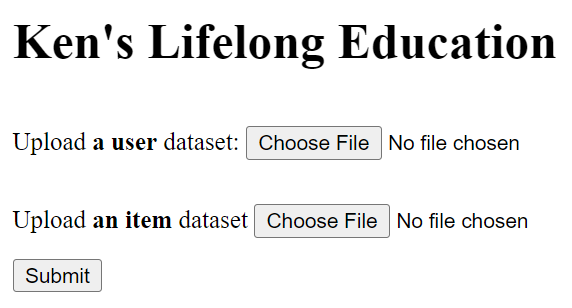
\includegraphics[width=4.2in]{img/dataset.png}
\caption{Uploading dataset}
\end{figure}

\newpage
\section{Input Data}
The input data of the recommendation system is a name of user who is considered to be recommended.
This person is typically a user who has taken at least one course on the platform.
The recommender is applied by 3 different techniques including of 1) TF-IDF and Linear Kernel 
approach 2) Feature Ratings and KNN approach, 3) the combination of 2 previous approaches.

\begin{figure}[H]
\center
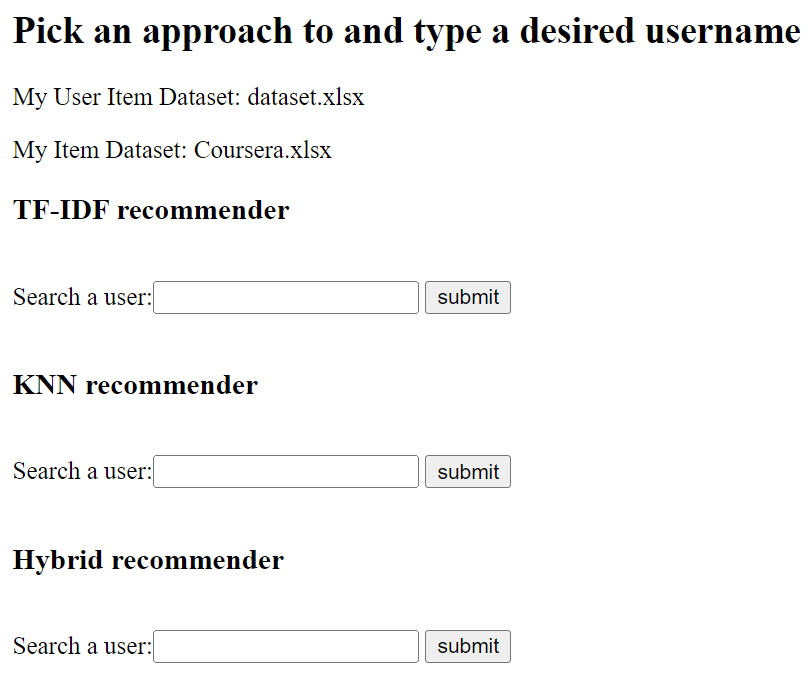
\includegraphics[width=6in]{img/input.png}
\caption{Input username}
\end{figure}

\newpage
\section{Output Data}
The output data of the recommendation system is a list of recommended courses for a given user. 
The list is sorted by the score of the suggestions, which is calculated by one of the 3 techniques.
The score is used to determine the relevance of the course to the user's profile.
\begin{figure}[H]
\center
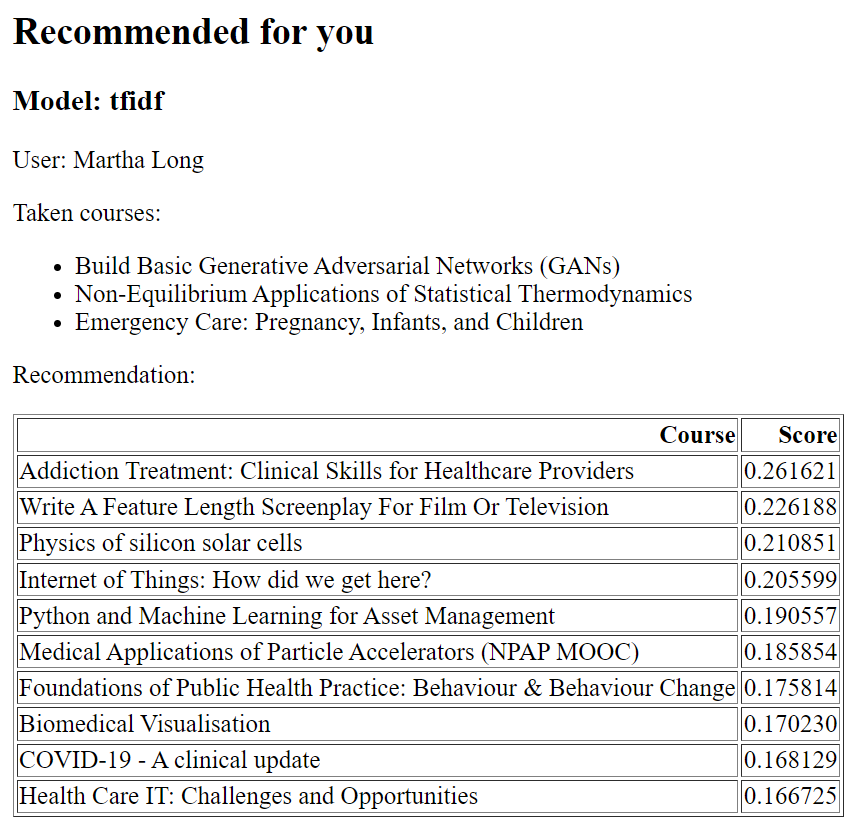
\includegraphics[width=6in]{img/output.png}
\caption{Output recommended courses}
\end{figure}

\section{evaluation outcomes}

We have selected the dataset to be used as follows
\begin{figure}[H]
\center
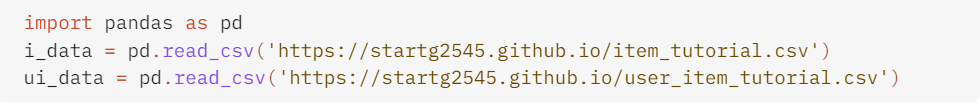
\includegraphics[width=6in]{img/Data.png}
\caption{Dataset to evaluation}
\end{figure}

\textbf{First approach}\\
This approach is an entire content-based filtering technique that leverages the Term Frequency and Inverse Document Frequency to statistically measure the importance of words in the descriptions.

The model achieved a Hit Rate accuracy of 14.69\%, signifying its effectiveness in predicting relevant items. Regarding the F1 Score, which balances precision and recall, the model attained an accuracy of 2.58\%, highlighting its overall performance in recommendation accuracy and error handling.

\textbf{Second Approach}\\
This approach involves using Feature Ratings and applying them to the K-Nearest Neighbors (KNN) algorithm in a recommendation system. However, this is a combination of content-based and collaborative filtering techniques.

The model attained a Hit Rate accuracy of 48.24\%, demonstrating its capability to predict relevant items. In terms of the F1 Score, which considers precision and recall, the model achieved an accuracy of 7.92\%, indicating its overall performance in recommendation accuracy and error management.

\textbf{Hybrid Approach}\\
The third approach combines TF-IDF content analysis with feature-based KNN, resulting in accurate and personalized recommendations for users.

The model achieved a Hit Rate accuracy of 69.18\%, indicating its effectiveness in predicting relevant items. The F1 Score, which balances precision and recall, stood at 11.62\%, reflecting its overall performance in recommendation accuracy and error minimization.